\documentclass[12pt]{article}
\usepackage[utf8]{inputenc}
\usepackage[czech]{babel}
\usepackage[left=2cm,text={17cm, 24cm},top=3cm,a4paper]{geometry}
\usepackage{times}
\usepackage{csquotes}
\usepackage[hidelinks, hyperfootnotes=false]{hyperref}
\usepackage{float}
\usepackage{multirow}
\usepackage{graphicx}
\begin{document}

\begin{titlepage}
\begin{center}

\Huge\textsc{Vysoké učení technické v Brně\\
\huge
Fakulta informačních technologií}\\
\vspace{\stretch{0.382}}
\LARGE ISA\\ 
\Huge Generování NetFlow dat\\ ze zachycené síťové komunikace\\
\Large MANUAL
\vspace{\stretch{0.618}}

\end{center}
\Large
30-10-2022 \hfill Václav Korvas (xkorva03)
\end{titlepage}

\tableofcontents
\newpage

\section*{Zadání}
Vytvořte aplikaci, která bude ze zachycených síťových dat ve formátu pcap vytvářet záznamy NetFlow, které následně odešle na kolektor, který je buď zadán příkazovou řádkou nebo se pošle na výchozí kolektor.
\\\\
Spuštění aplikace:\\ 
\\\texttt{./flow [-f <file>] [-c <netflow\_collector>[:<port>]] [-a <active\_timer>] [-i <inactive\_timer>] [-m <count>]}
\begin{itemize}
    \item {\texttt{-f <file>} jméno analyzovaného souboru nebo STDIN,}
    \item {\texttt{-c <neflow\_collector:port>} IP adresa, nebo hostname NetFlow kolektoru. Volitelně i UDP port (127.0.0.1:2055, pokud není specifikováno),}
    \item {\texttt{-a <active\_timer>} interval v sekundách, po kterém se exportují aktivní záznamy na kolektor (60, pokud není specifikováno),}
    \item {\texttt{-i <inactive\_timer>} - interval v sekundách, po jehož vypršení se exportují neaktivní záznamy na kolektor (10, pokud není specifikováno),}
    \item {\texttt{-m <count>} velikost flow-cache. Při dosažení max. velikosti dojde k exportu nejstaršího záznamu v cachi na kolektor (1024, pokud není specifikováno).\\}
\end{itemize}
Všechny parametry jsou brány jako volitelné. Pokud některý z parametrů není uveden, použije se místo něj výchozí hodnota.
\\\\
Upřesnění zadání: Program zpracuje vstupní argumenty, zpracuje vstupní soubor pokud byl zadán jinak čte ze stardartního vstupu a poté jednotlivé \uv{flows} odešle na specifikovaný kolektor. 
\\
\begin{itemize}
        \item {Jako export stačí použít NetFlow v5. Pokud byste implementovali v9 se šablonami, bude to bonusově zohledněno v hodnocení projektu,}
        \item {Pro vytváření flow stačí podpora protokolů TCP, UDP, ICMP,}
        \item {Informace, které neznáte (srcAS, dstAS, next-hop, aj.) nastavte jako nulové,}
        \item {Při exportování používejte původní časové značky zachycené komunikace,}
        \item {Exportované NetFlow data by měla být čitelná nástrojem nfdump.}
\end{itemize}
\pagebreak
\section{Návod na použití}
\subsection{Obsah oodevzdaného archivu}
\begin{itemize}
	\item {\texttt{Makefile}: s cíly \texttt{all} (sestaví výsledný program flow.cpp), \texttt{clean} (vymaže všechny vzniklé binární soubory a spustitelný program), \texttt{archive} (vytvoří archvive celého projektu),}
	\item {\texttt{manual.pdf}: soubor s programovou dokumentací,}
	\item {\texttt{flow.cpp}: zdrojový soubor výsledného programu,}
	\item {\texttt{flow.1}: manuálová stránka programu.}
\end{itemize}
\subsection{Rozbalení a použití}
První je nutné si tar-archiv rozbalit pomocí příkazu \texttt{tar -xvf xkorva03.tar}. Poté je nutné program přeloži pomocí příkazu \texttt{make} nebo
pomocí příkazu \texttt{make all}. Tímto vznikne spustitelný soubor v kořenové složce adresáře, ve kterém je spuštěn příkaz \texttt{make}. 
Po přeložení aplikace ji lze jednodušše spustit pomocí \texttt{./flow <argumenty>}, kde je možné uvést jednotlivé argumenty v libovolném pořadí.
\\\\ 
Ovšem pokud není zadán parametr \texttt{-f}, který určuje vstupní pcap soubor, ze kterého se bude číst, tak program bude číst ze standartního vstup neboli z \texttt{STDIN}.  
U parametru \texttt{-c}, kterým se určuje IPv4 nebo IPv6 adresu kolektoru. Ovšem je nutné při zadávání IPv6 adresy spolu s portem tuto adresu zadat následujícím způsobem: \texttt{[IPv6\_adresa]:port}. U adres IPv4 nebo doménového jména žádná taková omezení nejsou.
Při zadávaní IPv6 adresy bez portu žádné omezení není a lze ji zadat normálně a není nutné ji dát do hranatých závorek.
\\\\
Při nevalidním zadání vstupních argumentů končí program s návratovým chybovým kódem \texttt{1} a odpovídající chybovou hláškou.
\subsection*{Příklady spuštění}
Zde je uvedeno několik validních spuštění programu.
\begin{itemize}
	\item \texttt{./flow < icmp.pcap}
	\item \texttt{./flow -f icmp.pcap -c [::1]:2055}
	\item \texttt{./flow -f tcp.pcap -c ::1}
	\item \texttt{./flow -c 127.0.0.1:2055 < icmp.pcap}
	\item \texttt{./flow -f icmp.pcap -c localhost -m 5}
\end{itemize}
\pagebreak
\section{Teorie}
\subsection{Neflow}
NetFlow \cite{NT} je funkce, která umožňuje shromažďovat síťový provoz IP při vstupu nebo výstupu z rozhraní.
Analýzou dat poskytovaných NetFlow může správce sítě určit například zdroj a cíl provozu a příčiny přetížení. 
Typické nastavení monitorování toku se skládá ze tří hlavních součástí: \texttt{Flow exportér, Flow kolektor a aplikace pro analýzu}. Nás dále bude zajímat pouze flow exportér, protože to je hlavním cílem tohoto projektu.

\subsection{Netflow verze 5}
Cisco standart NetFlow verze 5 definuje tok (neboli flow) jako \texttt{jednosměrnou} sekvenci paketů. A tyto pakety mají sedm společných hodnot a tyto
hodnoty definují jednoznačný klíč pro tento tok. Tok je tedy identifikován násedující sedmicí: \texttt{vstupní rozhraní, zdrojová IP adresa, cílová IP adresa, protokol IP, 
zdrojový port\footnote{Zdrojový port je pouze pro protokoly TCP a UDP, u ostatních protokolů je to 0.}, cílový port\footnote{Port se uvádí pro protokoly UDP nebo TCP, pro protokol ICMP je to typ a kód, pro ostatní protokoly je to 0.}, typ služby IP}.
V našem případě vstupní rozhraní neznáme, jelikož provádíme pouze analýzu z pcap souboru, tedy tuto informaci vynecháváme a tok je definován zbylou šesticí.
Na obrázku \ref{picture} lze vidět co vše obsahuje hlavička jednotlivých toků a co se nachazí v těle lze najít zde \cite{NTv5}.
\begin{figure}[H]
	\begin{center}
	\scalebox{0.5}{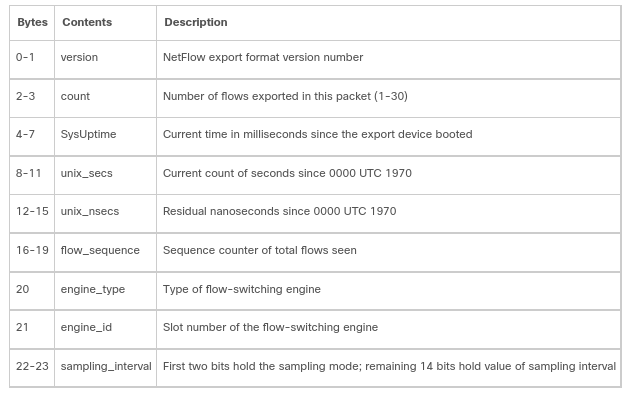
\includegraphics{hlavicka.png}}
	\caption{Hlavička NetFlow v5}
	\label{picture}
	\end{center}
\end{figure}
\subsection{Odesílaní toků}
V našem případě dochazí k exportu jednotlivých toků v následujících čtyřech případech. Zaprvé dochází k periodickému exportování toků vždy, když vyprší aktivní časovač. Poté pokud je některý z toků neaktivní delší dobu
než je specifikováno neaktivním časovačem. Zatřetí dojde k exportu nejstaršího záznamu v paměti pokud je paměť plná a posledním případem je ukončení relace TCP toku.
\pagebreak
\subsection{Analýza paketů}

\subsubsection{Ethernetový rámec}
V ethernetovém rámci má hlavička stále stejnou fixní velikost a to 14 bytů. Z techtě bytů je pro nás důležítá informace, která se nachází na posledních dvou bytech
a to je takzvaný Ethertype, neboli určení protokolu vyšší vrstvy. Tady nás bude zajímat pouze, zda-li se na vyšší vrstvě nachází IPv4 hlavička.

\subsubsection{Hlavička IPv4 paketu}
Hlavička IPv4 datagramu \cite{IPV4ICMP} má variabilní délku, proto je nutné její délku zjistit z pole \texttt{header length}, jenže toto číslo je nutné ještě vynásobit číslem 4, abychom dostali velikost hlavičky.
Další infomace, které nás zajímají je délka datagramu, typ protokolu, který se nachazí na vyšší vrstvě, zdrojová a cílová IP adresa a nakonec ješte ToS. 
Délka datagramu nás zajíma, protože je potřeba vědet velikost paketu bez ethernetového rámce a kontrolního součtu, který se někdy přikládá nakonec.

\subsubsection{TCP, UDP a ICMP}
TCP \cite{TCP}, UDP \cite{UDP} jsou protokoly operující na transportní vrstvě a nachazejí se nad IP datagramem. Z TCP a UDP datagramů budou důležité informace zdrojový a cílový port. Budou totiž sloužit k jednoznačné identifikaci jednotlivých záznamů toku.
\\\\
Z ICMP \cite{IPV4ICMP} hlavičky, která se nachází za hlavičkou IP, budeme potřebovat informace takzvaný ICMP kód a ICMP typ. Kde ICMP kód určuje o jaký typ se jedná (například echo nebo requst) a kód nám, ještě přesněji specifikuje typ ICMP zprávy.
Z těchto informací se poté vypočítá číslo, které se uloží jako cílový port a bude tak identifikovat tento tok. Vzorec pro výpočet je následující: \texttt{icmp\_type * 256 + icmp\_code}.

\pagebreak
\section{Implemtační detaily}
V následující sekci se popisuje strukturu programu a popisuje řešení některých nejduležitějších částí tohoto projektu.
V programu je hojně využita knihovna \texttt{pcap} a několik funkcí z této knihovny, jako třeba funkce na čtení pcap souboru nebo funkce
na vytvoření filtru, aby byly čteny pouze \texttt{ICMP, UDP} nebo \texttt{TCP} pakety. Všechny potřebné informace, jak použít tyto knihovní funkce byly z této stránky \cite{pcap}. 
\subsection*{Využité knihovny}
\begin{itemize}
	\item \texttt{pcap/pcap.h} - knihovna na zachytavání, procházení a filtrovaní paketů \cite{Pcapman}, 
	\item \texttt{getopt.h} - zpracování argumentů příkazové řádky \cite{ARG},
	\item \texttt{netinet/ether.h} - zpracování ethernetové hlavičky, 
	\item \texttt{sys/socket.h} - knihovna na otevírání síťových schránek,
	\item \texttt{netinet/ip\_icmp.h} - zpracování ICMP hlaviček paketů,
	\item \texttt{netinet/tcp.h} - zpracování TCP hlaviček paketů,
	\item \texttt{netinet/udp.h} - zpracování UDP hlaviček,
	\item \texttt{netdb.h} - překlad doménového jména na IP adresu,
	\item \texttt{netinet/ip.h} - zpracování IPv4 hlavičky.
\end{itemize}
\subsection{Parsování argumentů}
První věc, která se po spuštění programu provede, je zpracování argumentů z příkazové řádky. Toto se děje ve funkci \texttt{parse\_arguments}. V této funkci se k tomuto účelu používá funkce 
\texttt{getopt} z knihovny \texttt{getopt.h}. Pokud je použit neplatný argument program okamžite končí s návratovým kódem 1. 
\\\\
Postupně se pak kontrolují všechny argumenty a jejich parametry, například jestli soubor existuje nebo jestli bylo zadáno validní nezáporné číslo pro časovače.
Během průchodu všemi argumenty se postupně plní speciální struktura \texttt{arguments\_t}, ve které jsou uloženy všechny argumenty zadány uživatelem.

\subsection{Zpracovaní kolektoru}
Poté co jsou zpracovány všechny programové argumenty tak se volá funkce \texttt{parse\_collector}. V této funkci probíhá zpracování zadaného kolektoru uživatelem.
K tomuto účelu se používá funkce \texttt{inet\_pton} z knihovny \texttt{arpa/inet.h}. Nejprve se otestuje jestli je to validní IPv4 nebo IPv6 adresa bez portu, pokud ano
tak funkce končí úspěchem a do struktury \texttt{arguments\_t} si ukládá informaci, jestli se jednalo o IPv4 nebo IPv6 adresu.
\\\\
Pokud ovšem ani jedna z těchto funkci něuspěje tak se najde poslední \texttt{:} a cokoliv za ní se odstraní a je bráno jako číslo portu. A opět se otestuje, jestli je tato IP adresa validní.
Pokud ani toto neprojde tak zbývá poslední možnost a tou je, že uživatel zadal adresu kolektoru pomocí doménového jména.
Proto se doménové jméno zkusí přeložit pomocí funkce \texttt{getaddrinfo}. Poté se zjistí, jakou adresu nám tato funkce vrátila, tedy jestli se jedná o IPv4 nebo IPv6 adresu.
Pokud ani zde nedojde k úspechu tak funkce vrátí hodnotu 1 a běh programu se ukončí s korespondující chybovou hláškou.

\subsection{Zpracovaní paketů}
Po zpracovaní kolektoru, přichází na řadu čtení paketů z pcap souboru. K tomuto účelu slouží funkce \texttt{pcap\_open\_offline}, která buď čte ze specifikovaného souboru, nebo pokud místo souboru zadáme \texttt{-} tak čte ze standartního vstupu.
Dále následuje kontrola, že čteme ze souboru, který podporuje ethernetové hlavičky, pokud ne tak je program ukončen s chybovým kódem 1.
\\\\
Poté se vytvoří filtr, aby se vyfiltrovali nežádoucí protokoli, a my dostávali pouze pakety s protokoly \texttt{UDP, TCP a ICMP} a pouze IPv4. Poté tento filtr přeložíme pomocí funkce \texttt{pcap\_compile} a aplikujeme na vstupní soubor.
A nakonec se pak prochází přes všechny pakety funkcí \texttt{pcap\_loop} a pakety se čtou až dokud žádný není. A na každý paket se aplikuje funkce \texttt{process\_packet}.
\\\\
V této funkci se nejprve inicializuje struktura \texttt{nf\_v5\_body\_t}, která slouží k uchování informací ohledně jednotlivých toků. Poté dochází k extrakci důležitých informací
z jednotlivých vrstev a jejich ukládání do této struktury. Je to například zdrojová a cílová adresa, poté počet bytů, cilový a zdrojový port a protokolů UDP a TCP. U prvního paketu si
uložím jeho čas příchodu a považuji jej za systémový čas, který už nikdy neměním a je uložen v proměnné \texttt{first\_packet\_time}. A každý následující čas paketu je počítán relativně k tomuto času.

\subsection{Vytvaření a zpracování toků}
Po extrakci všech důležitých informací z hlaviček se volá funkce \texttt{process\_flow}. Zde se děje hned několik důležitých věcí a to: kontrola, jestli tok již existuje ve flow-cachi, pokud ne tak se vytvoří nový záznam toku a uloží se do cache. Poté zde probíha kontrola
jednotlivých podmínek, při jejichž porušení dochazí k exportování jednotlivých toků. Mezi tyto podmínky patři kontrola aktivního a neaktivního časovače, kontrola, jestli je plná cache nebo kontrola, zda-li jsme neobdrželi \texttt{FIN} nebo \texttt{RST} příznak v TCP hlavičce.
\subsection*{Kontrola existence flow záznamu}
Kontrola se provádí tak, že se iteruje skrz flow-cache. Flow-cache je implementována jako jednosměrně vázaný linearní seznam, kde každý tok je jednoznačně určena šesticí: \texttt{zdrojová a cílová IP adresa, zdrojový a cílový port, ToS a protokolem}.  
 Pokud takovýto záznam v cachi už existuje tak se pouze aktualizují položky jako \texttt{počet paketů, počet bytů ve flow, provede se kumulativní OR příznaků TCP, a aktualizuje se čas\\ příchodu posledního paketu flow}.
Pokud neexistuje tak se vytvoří nový záznam.

\subsection*{Přidání flow záznamu}
U přidávání nového záznamu se prvně provede kontrola, jestli náhodou není plná flow-cache, pokud ano tak se exportuje nejstarší záznam, tedy první prvek jednosměrně vázaného seznamu.
Pokud cache plná není tok se přidá do cache a nastaví se počet paketů této flow na 1. A vypočítá se čas prvího a posledního paketu tohoto toku vzhledem k prvnímu zpracovávanému paketu podle vzorce: 
\texttt{čas současného - čas prvního} a tento čas je v milisekundách. Tyto položky se uloží do políček \texttt{First a Last}, jedná se tedy o relativní čas vzhledem k prvnímu paketu.
\subsection*{Kontrola časovačů}
Kontrola časovačů probíha ještě před tím než se provede kontrola záznamu ve flow-cachi. Kontrola probíha tak, že se projde celá cache a nad každým záznamem se provede následujíci porovnání: vezme se aktualní čas zpracovávaného paketu odečte se od nej čas prvního paketu v dáné flow záznamu a porovná se jestli je větší než čas aktivního časovače.
Pokud ano tak se daný tok přidá do pole 30 záznamů, které se pak na konci procházení celé exportuje, protože lze najednou posílat až 30 záznamů.
\\\\
Pro neaktivní časovač se od aktualního času odečte čas posledního paketu v daném toku a pokud je větší než neaktivní časovač tak se daný tok opět uloží do pole, které se později exportuje.
\subsection*{Konrola příznaků TCP}
Úplně nakonci se provede ješte kontrola, jestli pravě zpracovávaný paket je typu TCP a pokud obsahuje příznak \texttt{FIN} nebo \texttt{RST} tak se přídá do daného toku, ke které patří a pak se celý tok exportuje.
\subsection{Odesílaní flows}
Odesílání jednotlivých flow záznamů probíhá ve funkci \texttt{send\_flow}, kde se prvně připraví flow k odeslání ve funkci \texttt{prepare\_flow}. V této funkci se alokuje dostatečně veliká pamět pro všechny flow i s hlavičkou, která je definována ve struktuře
\texttt{nf\_v5\_header\_t}. Tato hlavička se naplní informacemi, které se převedou pomocí \texttt{htons a htonl} do síťového formátu. A to stejné se provede s informacemi v jednotlivých flow záznamech.
\\\\
Poté funkce vratí alokovaný a naplněný buffer. Dále se otevře buď IPv4 nebo IPv6 schránka. A poté se na danou IP adresu a port pošle tento buffer pomocí funkce \texttt{sendto()}.
\section{Testování}
Testování bylo prováděno manuálně za pomocí nástrojů \texttt{wireshark \cite{wire}, nfdump \cite{DUMP} a\\ nfcapd \cite{CAPD}}. Kdy jsme si první v nástroji wireshark odchytil komunikaci a tu vyexportoval do souboru
pcap. Následně byl spuštěn nástroj nfcapd následujícím příkazem: \texttt{nfcapd -D -T all -l ~/logs -I any -S 2 -p 2055 -t 60}, který zachytává netflow komunikaci na portu 2055 a ukládá ji do souboru.
A poté byl spušten program, kde na vstupu byl vygenerovaný soubor pcap. A nakonec byla komunikace zobrazena pomocí nástroje nfdump: \texttt{nfdump -r logs/2022/*}. Dodatečně bylo ověřeno, že nástroj wireshark zachytil odeslaný paket bez chyby.
\begin{figure}[H]
	\begin{center}
	\scalebox{0.6}{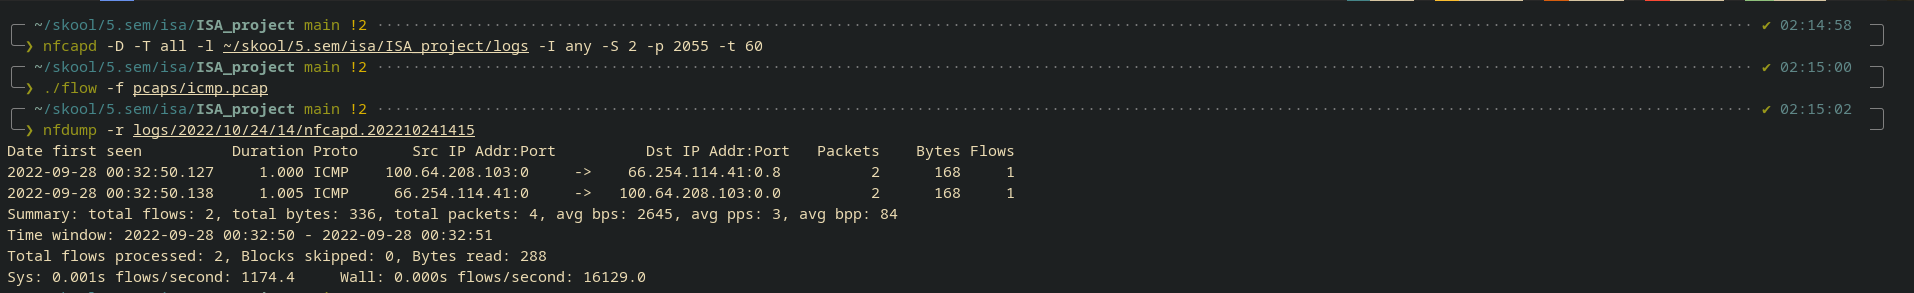
\includegraphics{nfutils.png}}
	\caption{Ukázka spuštění jednotlivých programů a výstupu nástroje nfdump.}
	\label{fig:picture1}
	\end{center}
\end{figure}
\begin{figure}[H]
	\begin{center}
	\scalebox{0.5}{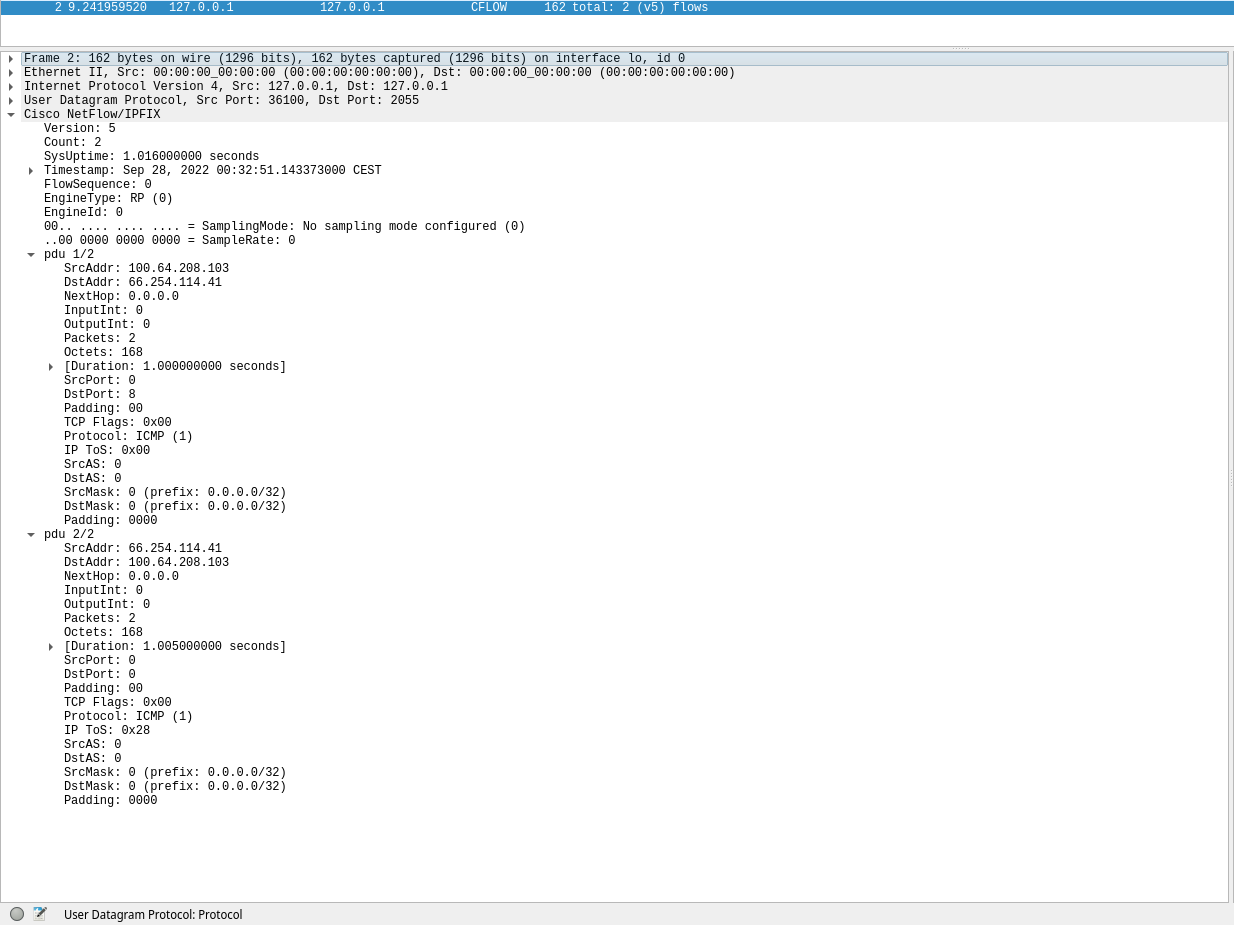
\includegraphics{wireshark.png}}
	\caption{Zachycený paket nástrojem wireshark.}
	\label{fig:picture2}
	\end{center}
\end{figure}
\pagebreak
\begin{thebibliography}{plain}
  \bibitem[1]{pcap} Carstens, T., Guy, H..
	  \emph{Programming with pcap} [online]. 2022. \\
		Dostupné z: \href{https://www.tcpdump.org/pcap.html}{\texttt{https://www.tcpdump.org/pcap.html}}
	\bibitem[2]{NTv5} Cisco Systems.
	  \emph{NetFlow Datagram Format} [online]. Dokumentace Cisco; 2014-09-17.\\ 
		Dostupné z: \href{https://en.wikipedia.org/wiki/OSI\_model}{\texttt{www.cisc.comwww.cisco.com/c/en/us/td/docs/net\_mgmt/netflow\\\_collection\_engine}}
	\bibitem[3]{IPV4ICMP} Veselý, V. 
		\emph{Síťová vrstva -- ICMP} [Univerzitní přednáška]. 2021. \\ 
		Dostupné z: \href{https://wis.fit.vutbr.cz/FIT/st/cfs.php.cs?file=\%2Fcourse\%2FIPK-IT\%2Flectures\%2FIPK2021-06-IPv6.pdf&cid=14678}{\texttt{https://wis.fit.vutbr.cz/FIT/st/cfs.php.cs?file=\%2Fcourse\\\%2FIPK-IT\%2Flectures\%2FIPK2021-06-IPv6.pdf\&cid=14678}}
	\bibitem[4]{TCP} Wikipedia contributors.
	  \emph{Transmission Control Protocol} [online]. Wikipedia, The Free Encyclopedia; 2022-04-09.\\ 
		Dostupné z: \href{https://en.wikipedia.org/wiki/Transmission\_Control\_Protocol}{\texttt{https://en.wikipedia.org/wiki/Transmission\_Control\_Protocol}}
	\bibitem[5]{UDP} Wikipedia contributors.
	  \emph{User Datagram Protocol} [online]. Wikipedia, The Free Encyclopedia; 2022-03-24. \\
		Dostupné z: \href{https://en.wikipedia.org/wiki/User\_Datagram\_Protocol}{\texttt{https://en.wikipedia.org/wiki/User\_Datagram\_Protocol}}
	\bibitem[6]{ARG} Free Software Foundation. 
		\emph{getopt(3) — Linux manual page} [online].\\
		Dostupné z: \href{https://www.man7.org/linux/man-pages/man3/getopt.3\\.html}{\texttt{https://www.man7.org/linux/man-pages/man3/getopt.3.html}}
	\bibitem[7]{wire} Combs, G. 
		\emph{Wireshark} [online] 2022.
		Dostupné z: \href{https://www.wireshark.org/}{\texttt{https://www.wireshark.org/}}
	\bibitem[8]{NT} Wikipedia contributors.
	  \emph{NetFlow} [online]. Wikipedia, The Free Encyclopedia; 2022-04-09.\\ 
		Dostupné z: \href{https://en.wikipedia.org/wiki/NetFlow}{\texttt{https://en.wikipedia.org/wiki/NetFlow}}
	\bibitem[9]{DUMP} Free Software Foundation. 
		\emph{nfdump(1) — FreeBSD manual page} [online].\\
		Dostupné z: \href{https://www.freebsd.org/cgi/man.cgi?query=nfdump&apropos=0&sektion=1&manpath=FreeBSD+8.2-RELEASE+and+Ports&format=html}{\texttt{https://www.freebsd.org/cgi/man.cgi?query=nfdump}}
	\bibitem[10]{CAPD} Free Software Foundation. 
		\emph{nfcapd(1) — FreeBSD manual page} [online].\\
		Dostupné z: \href{https://www.freebsd.org/cgi/man.cgi?query=nfcapd&apropos=0&sektion=1&manpath=FreeBSD+8.2-RELEASE+and+Ports&format=html}{\texttt{https://www.freebsd.org/cgi/man.cgi?query=nfcapd}}
	\bibitem[11]{Pcapman} Jacobson, V., et al. 
		\emph{Man page of pcap} [online], 2020-09-09.\\
		Dostupné z: \href{https://www.tcpdump.org/manpages/pcap.3pcap.html}{\texttt{https://www.tcpdump.org/manpages/pcap.3pcap.html}}

  \end{thebibliography}
\end{document}